\documentclass[10pt,a4paper]{article}
\usepackage[utf8]{inputenc}
\usepackage[english]{babel}
\usepackage{amsmath}
\usepackage{amsfonts}
\usepackage{amssymb}
\usepackage{graphicx}
\usepackage[left=2cm,right=2cm,top=2cm,bottom=2cm]{geometry}
\usepackage{physics}
\usepackage{tikz}
\usepackage{stmaryrd}

\author{Marco Biroli}
\title{Graphene and Haldane model}

\begin{document}

\maketitle

\section{Graphene and Dirac points.}

\begin{enumerate}
\item  We have that:
\[
\vb{\delta_1} = (0, a) \mbox{~~and~~} \vb{\delta_2} = \frac{d}{2} (\sqrt{3}, -1) \mbox{~~and~~} \vb{\delta_3} = \frac{d}{2} (-\sqrt{3}, -1)
\]
Then we have that:
\begin{align*}
f_{\vb{k}} &= - t \exp(-\frac{i d}{2} (\sqrt{3} k_x + k_y)) \left( 1 + \exp(i \sqrt{3} d k_x) + \exp(\frac{i d}{2} (\sqrt{3} k_x + 3 k_y)) \right) \\
&= - t\left[ \underbrace{\left( 2 \cos(\frac{\sqrt{3}}{2} d k_x) \cos(\frac{d}{2} k_y) + \cos(d k_y) \right)}_{h_1} + i \underbrace{2 \left( \cos(\frac{\sqrt{3}}{2} d k_x) - \cos(\frac{d}{2} k_y) \right) \sin(\frac{d}{2} k_y)}_{h_2}
 \right]
\end{align*}
And taking $h_3 = 0$ we have that:
\[
H = -t \, \, \vb{h}_{\vb{k}} \cdot \vb{\sigma}
\]
Notice that without expanding the terms we can also simply write:
\[
H = \sum_{i = 1}^3 \left( \cos(\vb{k} \cdot \vb{\delta_i} ) \sigma_x + \sin(\vb{k} \cdot \vb{\delta_i}) \sigma_y \right)
\]
Then notice that similarly as in the TD we have that:
\[
H^2 = t^2 || \vb{h}_{\vb{k}} ||^2 \text{ Id}
\]
Thus the eigenvalues of $H$ are given by:
\[
E_\pm = \pm t || \vb{h_{\vb{k}}} || = \pm t \sqrt{3 + 2 \cos(d k_x \sqrt{3}) + 2 \cos(\frac{d}{2} (k_x\sqrt{3} - 3 k_y)) + 2 \cos(\frac{d}{2}(k_x\sqrt{3} + 3k_y))}
\]
Notice that solving for $E_\pm = 0$ we get indeed the Dirac point $K$, as well as $-K$ or $(K_x, - K_y)$ for example. Plotting the energy spectrum we obtain Figure \ref{eigenplot}.
\begin{figure} \label{eigenplot}
\centering
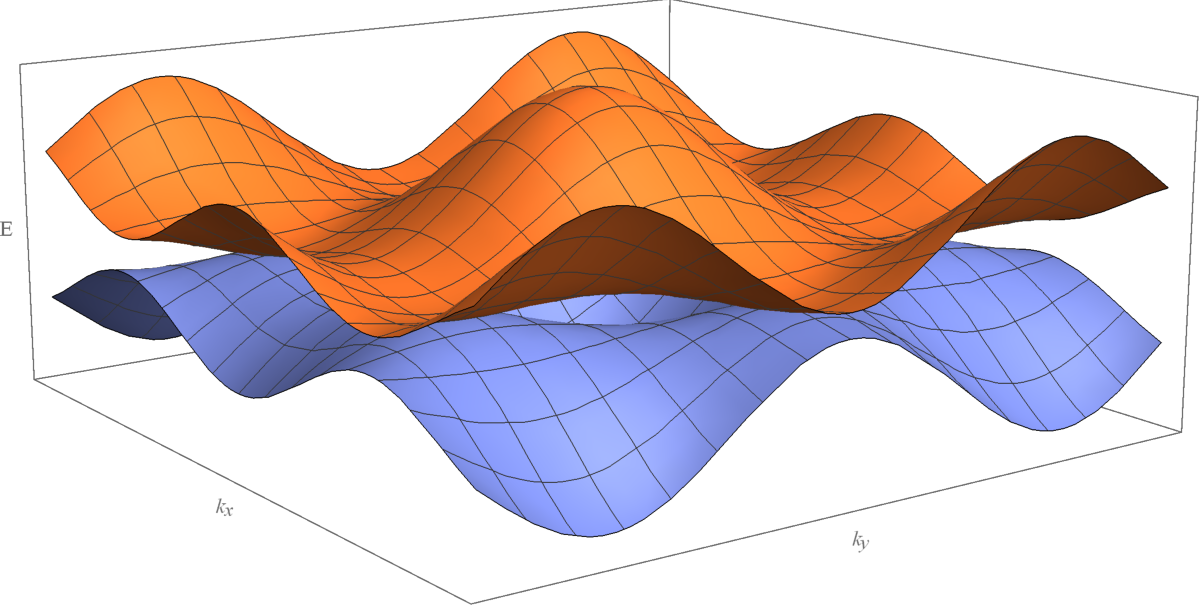
\includegraphics[width = 0.5\textwidth]{energylevels}
\caption{Plot of the positive energy levels for $k_x, k_y \in [-\frac{\pi}{d}, \frac{\pi}{d}]$.}
\end{figure}

\item We write $\vb{k} = \vb{K} + \vb{\varepsilon}$. Then we know that $H_{\vb{K}} = 0$ and $f_{\vb{K}} = 0$ hence we have that:
\[
f_{\vb{k}} = f_{\vb{K}}  + \frac{1}{2}\vb{\varepsilon} \cdot \left(\grad f_{\vb{k}} \right) \Big|_{\vb{k} = \vb{K}} = \frac{1}{2} \vb{\varepsilon} \cdot \left( \frac{3 d t}{2}, - \frac{3}{2} i d t  \right) = \frac{3dt}{4}\left( \varepsilon_x - i \varepsilon_y \right)
\] 
Hence we also get the linearization of $\vb{h}$ easily as:
\[
\vb{h}_{\vb{k}} = \left(\frac{3dt}{4} (k_x - K_x), -\frac{3 dt}{4} (k_y - K_y)\right)  = \frac{3 dt}{4}\left(\varepsilon_x, - \varepsilon_y \right)
\]
And hence:
\[
E_\pm = \pm t \frac{3 dt}{4} \sqrt{\varepsilon_x^2 + \varepsilon_y^2} = \pm \frac{3 d t}{4} r 
\]

\item Close to $\vb{K}$ the Hamitlonian reads:
\[
H = \frac{3 d t}{4}\begin{pmatrix}
0 & \varepsilon_x + i \varepsilon_y\\
\varepsilon_x - i \varepsilon_y & 0 
\end{pmatrix}
\]
Hence we have that the eigenvectors are given by:
\[
u_{\pm \vb{k}} = \begin{pmatrix}
\pm \sqrt{\varepsilon_x^2 + \varepsilon_y^2}\\
\varepsilon_x - i \varepsilon_y
\end{pmatrix} = \begin{pmatrix}
\pm \varepsilon\\
e^{-i \theta}
\end{pmatrix} = \begin{pmatrix}
\pm \varepsilon e^{i \theta}\\
1 
\end{pmatrix}
\]
Where we took:
\[
\cos \theta = \frac{\varepsilon_x}{\varepsilon} \mbox{~~and~~} \sin \theta = \frac{\varepsilon_y}{\varepsilon} \mbox{~~and~~} \varepsilon = \sqrt{\varepsilon_x^2 + \varepsilon_y^2}
\]

Hence we get:
\[
\mathcal{A}_{\pm x} = u_\mp^T \pdv{}{k_x} u_\pm = \begin{pmatrix}
\mp \sqrt{\varepsilon_x^2 + \varepsilon_y^2} & \varepsilon_x - i \varepsilon_y 
\end{pmatrix}  \begin{pmatrix}
\pm \frac{\varepsilon_x}{\sqrt{\varepsilon_x^2 + \varepsilon_y^2}}\\
\varepsilon_x + K_x
\end{pmatrix} = - \varepsilon_x + (\varepsilon_x - i \varepsilon_y) (\varepsilon_x + K_x)
\]
Similarly we get:
\[
\mathcal{A}_{\pm y} = u_\mp^T \pdv{}{k_y} u_\pm = \begin{pmatrix}
\mp \sqrt{\varepsilon_x^2 + \varepsilon_y^2} & \varepsilon_x - i \varepsilon_y 
\end{pmatrix}  \begin{pmatrix}
\pm \frac{\varepsilon_y}{\sqrt{\varepsilon_x^2 + \varepsilon_y^2}}\\
- i \varepsilon_y
\end{pmatrix} = - \varepsilon_y - \varepsilon_y (i\varepsilon_x + \varepsilon_y) = -\varepsilon_y(1 + i \varepsilon_x + \varepsilon_y)
\]
Taking $\varepsilon_x = \varepsilon \cos(\theta)$ and $\varepsilon_y = \varepsilon \sin(\theta)$ and replacing above we get:
\[
\mathcal{A}_\pm = \begin{pmatrix}
\frac{\varepsilon}{2}(1 - e^{i\theta} + e^{-i\theta}(1 + 2 K_x) + e^{-2i\theta}\\ 
-\frac{\varepsilon}{2i}(e^{i \theta} - e^{-i\theta})(1 + \varepsilon e^{i \theta}) 
\end{pmatrix}
\]

\item We therefore get for the integral:
\[
\varphi_\mathcal{A} = \int_0^{2\pi} \mathcal{A}_{\pm} \cdot \begin{pmatrix}
\cos\theta\\
\sin\theta
\end{pmatrix} \varepsilon  \dd \theta
\]

\section{draft}
Now for simplicity we write $r e^{i \theta} =  \varepsilon_x + i \varepsilon_y$ where $r  = \sqrt{\varepsilon_x^2 + \varepsilon_y^2}$ and $\theta = \arctan(\varepsilon_y/\varepsilon_x)$. Then we can rewrite the above as:
\[
H = \frac{3 r dt }{4} \begin{pmatrix}
0 & e^{i\theta}
e^{- i \theta} & 0
\end{pmatrix}
\] 
Which immediately tells us that:
\[
E_\pm = \pm \frac{3 r d t}{4} \mbox{~~and~~} u_{\pm} = \begin{pmatrix}
\pm e^{i \theta}\\
1
\end{pmatrix}
\]


\end{enumerate}
\end{document}